\documentclass[11pt]{article}
\usepackage{acl2015}
\usepackage{times}
\usepackage{url}
\usepackage{latexsym}
\usepackage{graphicx}
\usepackage{booktabs}
\usepackage{makecell}
\usepackage{graphicx}
\graphicspath{ {images/} }

\renewcommand\theadalign{bc}

\title{Authorship Attribution of the Federalist Papers using Recurrent Neural Network Language Models}

\author{Jason Harville \\
  \small School of Information \\
  \small University of California, Berkeley\\
  \small Berkeley, CA 94720 \\
  {\tt \small jlharville@berkeley.edu} \\\And
  Shawn Kessler \\
  \small School of Information \\
  \small University of California, Berkeley\\
  \small Berkeley, CA 94720 \\
  {\tt \small skessler@berkeley.edu} \\\And
  Mehdi Saedi \\
  \small School of Information \\
  \small University of California, Berkeley\\
  \small Berkeley, CA 94720 \\
  {\tt \small msaedi@berkeley.edu} \\}

\date{12/19/2017}

\begin{document}
\maketitle
\begin{abstract}
  We show that authorship attribution can be accomplished with a fairly small corpus and cutting-edge neural network algorithms given narrow constraints. In particular, we look at the disputed Federalist Papers and try to match state-of-the-art non-neural-network machine learning analysis of the papers using a recurrent neural network language model (RNNLM).
\end{abstract}

\section{Introduction}

Authorship attribution, a classification problem that seeks to determine the author of a given document or shorter text string, has a long and rich history~\cite{Stamatatos:08}. One of the earliest attempts to mathematically determine authorship is Mosteller and Wallace’s use of Bayesian analysis of word frequency in the Federalist Papers to determine the authorship of disputed papers~\cite{Mosteller:63}. The Federalist Papers are a collection of writings in support of the newly-proposed American Constitution, published between 1787-1788. Three authors, James Madison, Alexander Hamilton, and John Jay~\shortcite{Haminlton:87}, wrote the papers but published under the same pseudonym, leading to uncertainty over who authored which papers. To date, the authorship of 15 of the 85 papers is still disputed. Hamilton published the set and laid claim to 15 of the papers that Madison later published and claimed were in fact written by him, not Hamilton. Hamilton was dead at this point and so no further reconciliation could be made except by third parties using authorship attribution techniques.

\section{Background}
Since the work of Mosteller and Wallace, the Federalist Papers have been commonly used as a reference corpus for authorship attribution. While neural-network-based models have gained prominence in natural language processing, we have been unable to find examples of neural network techniques applied to this important benchmark corpus. The latest work on the Federalist Papers we could find was by Jockers and Witten in 2010; they compared multiple machine learning algorithms that were state of the art at the time~\cite{Jockers:10}. We proposed exploring various neural network techniques to the Federalist Papers in order to benchmark them against previous techniques on the known papers and make our own predictions on authorship of the disputed papers. In particular, we explored Neural Network Language Models outlined in Zhenhao Ge, Yufang Sun and Mark J.T. Smith~\shortcite{GeAll:16}, and Zhenhao Ge, Yufang Sun~\shortcite{Ge:16}.

\begin{table*}[t]
	\centering
	\begin{tabular}{lrrrr}
	\toprule
	\bf Author&   \bf Words & \bf Sentences & \bf \thead{Words /\\ Sentences} & \bf \thead{Vocabulary Size\\ (Original / Processed)} \\
	\midrule
	Alexander Hamilton &  1,512,817 &     62,612 &        24.2 & 26,437 / 20,693 \\
	Benjamin Franklin  &    70,199 &      2,523 &        27.8 &   7,688 / 7,029 \\
	George Washington  &    19,903 &       674 &        29.5 &   3,329 / 3,075 \\
	James Madison      &  1,583,467 &    100,068 &        15.8 & 27,005 / 19,113 \\
	James Monroe       &    45,597 &      1,449 &        31.5 &   4,147 / 3,764 \\
	John Adams         &   168,191 &      66,04 &        25.5 &  12,568 / 1,622 \\
	John Jay           &     8,374 &       199 &        42.1 &   1,754 / 1,566 \\
	Thomas Jefferson   &  2,888,245 &    136,333 &        21.2 & 37,796 / 33,649 \\
	Thomas Paine       &   364,912 &     14,224 &        25.7 & 18,251 / 11,725 \\
	\bottomrule
	\end{tabular}
	\caption{\label{corpus} Larger corpus details}
\end{table*}
\section{Data Preparation}
We pulled the Federalist Papers from the Gutenberg Project. However, to create good word embeddings, we suspected we would require a much bigger corpus. To compensate for the relatively small size of the federalist papers and for more-diverse experimentation, we explored other sources such as other documents written by the three suspected authors as well as other books, short stories, and essays from the same time period and also pulled a substantial number of documents from contemporary authors with extensive writings and/or involvement in the founding of early-American government. We prioritized finding other sources in the following order:
\begin{enumerate}
	\item Anything written by James Jay, Alexander Hamilton, or James Madison (in any year)
	\item Anything written by a founding father or major American political figure from 1760 to 1810
	\item Any non-fiction by an American author written between 1760 and 1810
	\item Any fiction by an American author written between 1760 and 1810
\end{enumerate}
We tried to keep that range of years generally narrow to avoid capturing changes in usage of American English over time. A substantial number of documents were letters from one of the founding fathers to a political figure or vice versa. To reduce the influence of names on author classification, both sender and recipient names were omitted in our data preparation process. Table \ref{corpus} lists more details on the larger corpus used.

\begin{table*}[t]
	\centering
	\resizebox{\textwidth}{!}{\begin{tabular}{lllllllllll}
			\toprule
			\bf Paper & \bf NSC raw & \bf SVM raw & \bf KNN raw & \bf Delta raw & \bf RDA raw & \bf NSC pp & \bf SVM pp & \bf KNN pp & \bf Delta pp & \bf RDA pp\\
			\midrule
			No. 18 & Madison & Madison & Madison & Madison & Madison & Madison & Madison & Hamilton & Madison & Madison \\ 
			No. 19 & Madison & Madison & Hamilton & Madison & Madison & Madison & Madison & Hamilton & Madison & Madison \\ 
			No. 20 & Madison & Madison & Madison & Madison & Madison & Madison & Madison & Hamilton & Madison & Madison \\ 
			No. 49 & Madison & Madison & Madison & Madison & Madison & Madison & Madison & Hamilton & Madison & Madison \\ 
			No. 50 & Madison & Madison & Madison & Madison & Madison & Madison & Madison & Madison & Hamilton & Madison \\ 
			No. 51 & Madison & Madison & Hamilton & Madison & Madison & Madison & Madison & Madison & Madison & Madison \\ 
			No. 52 & Madison & Madison & Hamilton & Madison & Madison & Madison & Madison & Madison & Madison & Madison \\ 
			No. 53 & Madison & Madison & Madison & Madison & Madison & Madison & Madison & Madison & Madison & Madison \\ 
			No. 54 & Madison & Hamilton & Madison & Madison & Madison & Madison & Madison & Hamilton & Madison & Madison \\ 
			No. 55 & Madison & Hamilton & Madison & Madison & Hamilton & Madison & Madison & Madison & Madison & Hamilton \\ 
			No. 56 & Madison & Madison & Hamilton & Madison & Madison & Madison & Madison & Madison & Madison & Madison \\ 
			No. 57 & Madison & Hamilton & Hamilton & Madison & Madison & Madison & Madison & Hamilton & Madison & Madison \\ 
			No. 58 & Madison & Madison & Madison & Madison & Madison & Madison & Madison & Madison & Madison & Madison \\ 
			No. 62 & Madison & Madison & Madison & Madison & Madison & Madison & Madison & Madison & Madison & Madison \\ 
			No. 63 & Madison & Madison & Madison & Madison & Madison & Madison & Madison & Madison & Madison & Madison \\ 
			\bottomrule
		\end{tabular}}
		\caption{\label{attributions by method} ML State of the Art Analysis Results\footnotemark}
	\end{table*}
\section{Methods}
The RNNLM we used is a slightly modified version of the long-term short-term (LSTM) + embedding layer model completed in Assignment 4. We altered this model to be a classifier rather than a sequence generator. To effect this change, we used the authors as classes - rather than every word in the vocabulary - and we used only the loss from the very last word in the sequence for back propagation. In addition we had to alter the batch generator to properly create a set of $y$ values, where each $y$ value was an author ID, rather than the next word in the sequence. We continued with fixed-length sequences of words for training and testing, not variable length sentences.\\
Our first attempt found us training on our larger corpus. It was apparent that the RNNLM model preferred the author with the most data, resulting in it picking Thomas Jefferson quite often for the author of many of the disputed and undisputed Federalist Papers. A crucial point we learned here is that the batch composition is very important. We created batches that contained all of the same author and fed them into the model such that an epoch would end with multiple batches for the same author. This caused the classifier to always pick the last author trained on as the author of all papers. We implemented what we thought was a fix by mingling batches so that batch order was random, but each batch still only contained a single author. This fixed the immediate problem of always picking the last author trained, but Thomas Jefferson was still the preferred author. We discovered the right way to create a batch is to think of it as a random experiment: the content of the batch needs to closely match the distribution of the overall population. After randomly commingling authors in a single batch, we started to see more consistent predictions but still a bias toward Jefferson. The model was also predicting Hamilton and Madison as authors of some of the documents. However, they had the second- and third-most sequences in the corpus following Thomas Jefferson, so it was not obvious if the model was calculating useful weights based on the authors' writing styles or if it was still simply basing its results on which classes it was seeing most often during training.\\
To confirm our model worked on a corpus balanced across authors, we scaled training data down to three papers, one that was known to be authored by each of the three authors of the Federalist Papers. We then overfit the model on these three papers and confirmed that it always predicted the correct author for the three training papers with about 98\% certainty.\\
We slowly added more data back in, starting with the federalist papers. Once we had all of them in, without the data from the larger corpus, we saw predictions that were a lot more sane. In this setting, the model never once predicted John Jay as the author of one of the disputed papers, and Jefferson was not even an option. However, John Jay wrote a much smaller number of papers compared to his compatriots, so we still were not certain the model was not predicting based mostly on number of samples. We scaled our data down one more time. This time we included all of John Jay's papers and enough of Hamilton and Madison's papers to roughly match the size of John Jay's papers. With this small balanced corpus, the system still never selected John Jay as a potential author. Finally we felt confidence in our model and we decided to drop John Jay from the equation to focus on Madison vs. Hamilton. We used all of their undisputed papers and updated the model to have only two classes.\\
We split the undisputed papers into a training set and a test set. Once the model was 96\% accurate on the test set we looked at what it predicted for the disputed papers. It was giving Hamilton more credit than most historians and our baseline did. However, Hamilton had many more papers than Madison in our training set. We trimmed down the number of Hamilton papers so that the training set and test set included a similar number of text by both authors, with a total of 2824 sequences each comprised of fifteen words in our training set. After training the model until it again achieved at least 95\% accuracy, it predicted all but three of the disputed documents as Madison’s (12 of 15). This is the sort of ratio we expected. We experimented with a few different parameters: embedded feature size, number of layers, learning rate, word segment length. One hundred embedded features, with 1 layer, .08 learning rate, and 15 word long segments gave us the best cross-validation results.\\
As a baseline, we used other state-of-the-art ML based assessments of the Federalist Papers. Our results are similar to Jockers and in particular do not include John Jay as a possible author.\\
We also experimented with a Naive Bayes bag-of-words (BOW) classifiers. We trained the models with and without removing English stop-words and with and without tf-idf weighting, resulting in four different classifiers. We trained the models on both the training set described above  and on the entire set of federalist papers with known authorship, and in both cases used the trained models to predict the authors of the unknown papers.
\footnotetext{From Matthew L. Jockers, and Daniela M. Witten, A comparative study of machine learning methods for authorship attribution, Literary and Linguistic Computing, 215-223 (2010).}

\begin{figure*}[h]
	\centering
	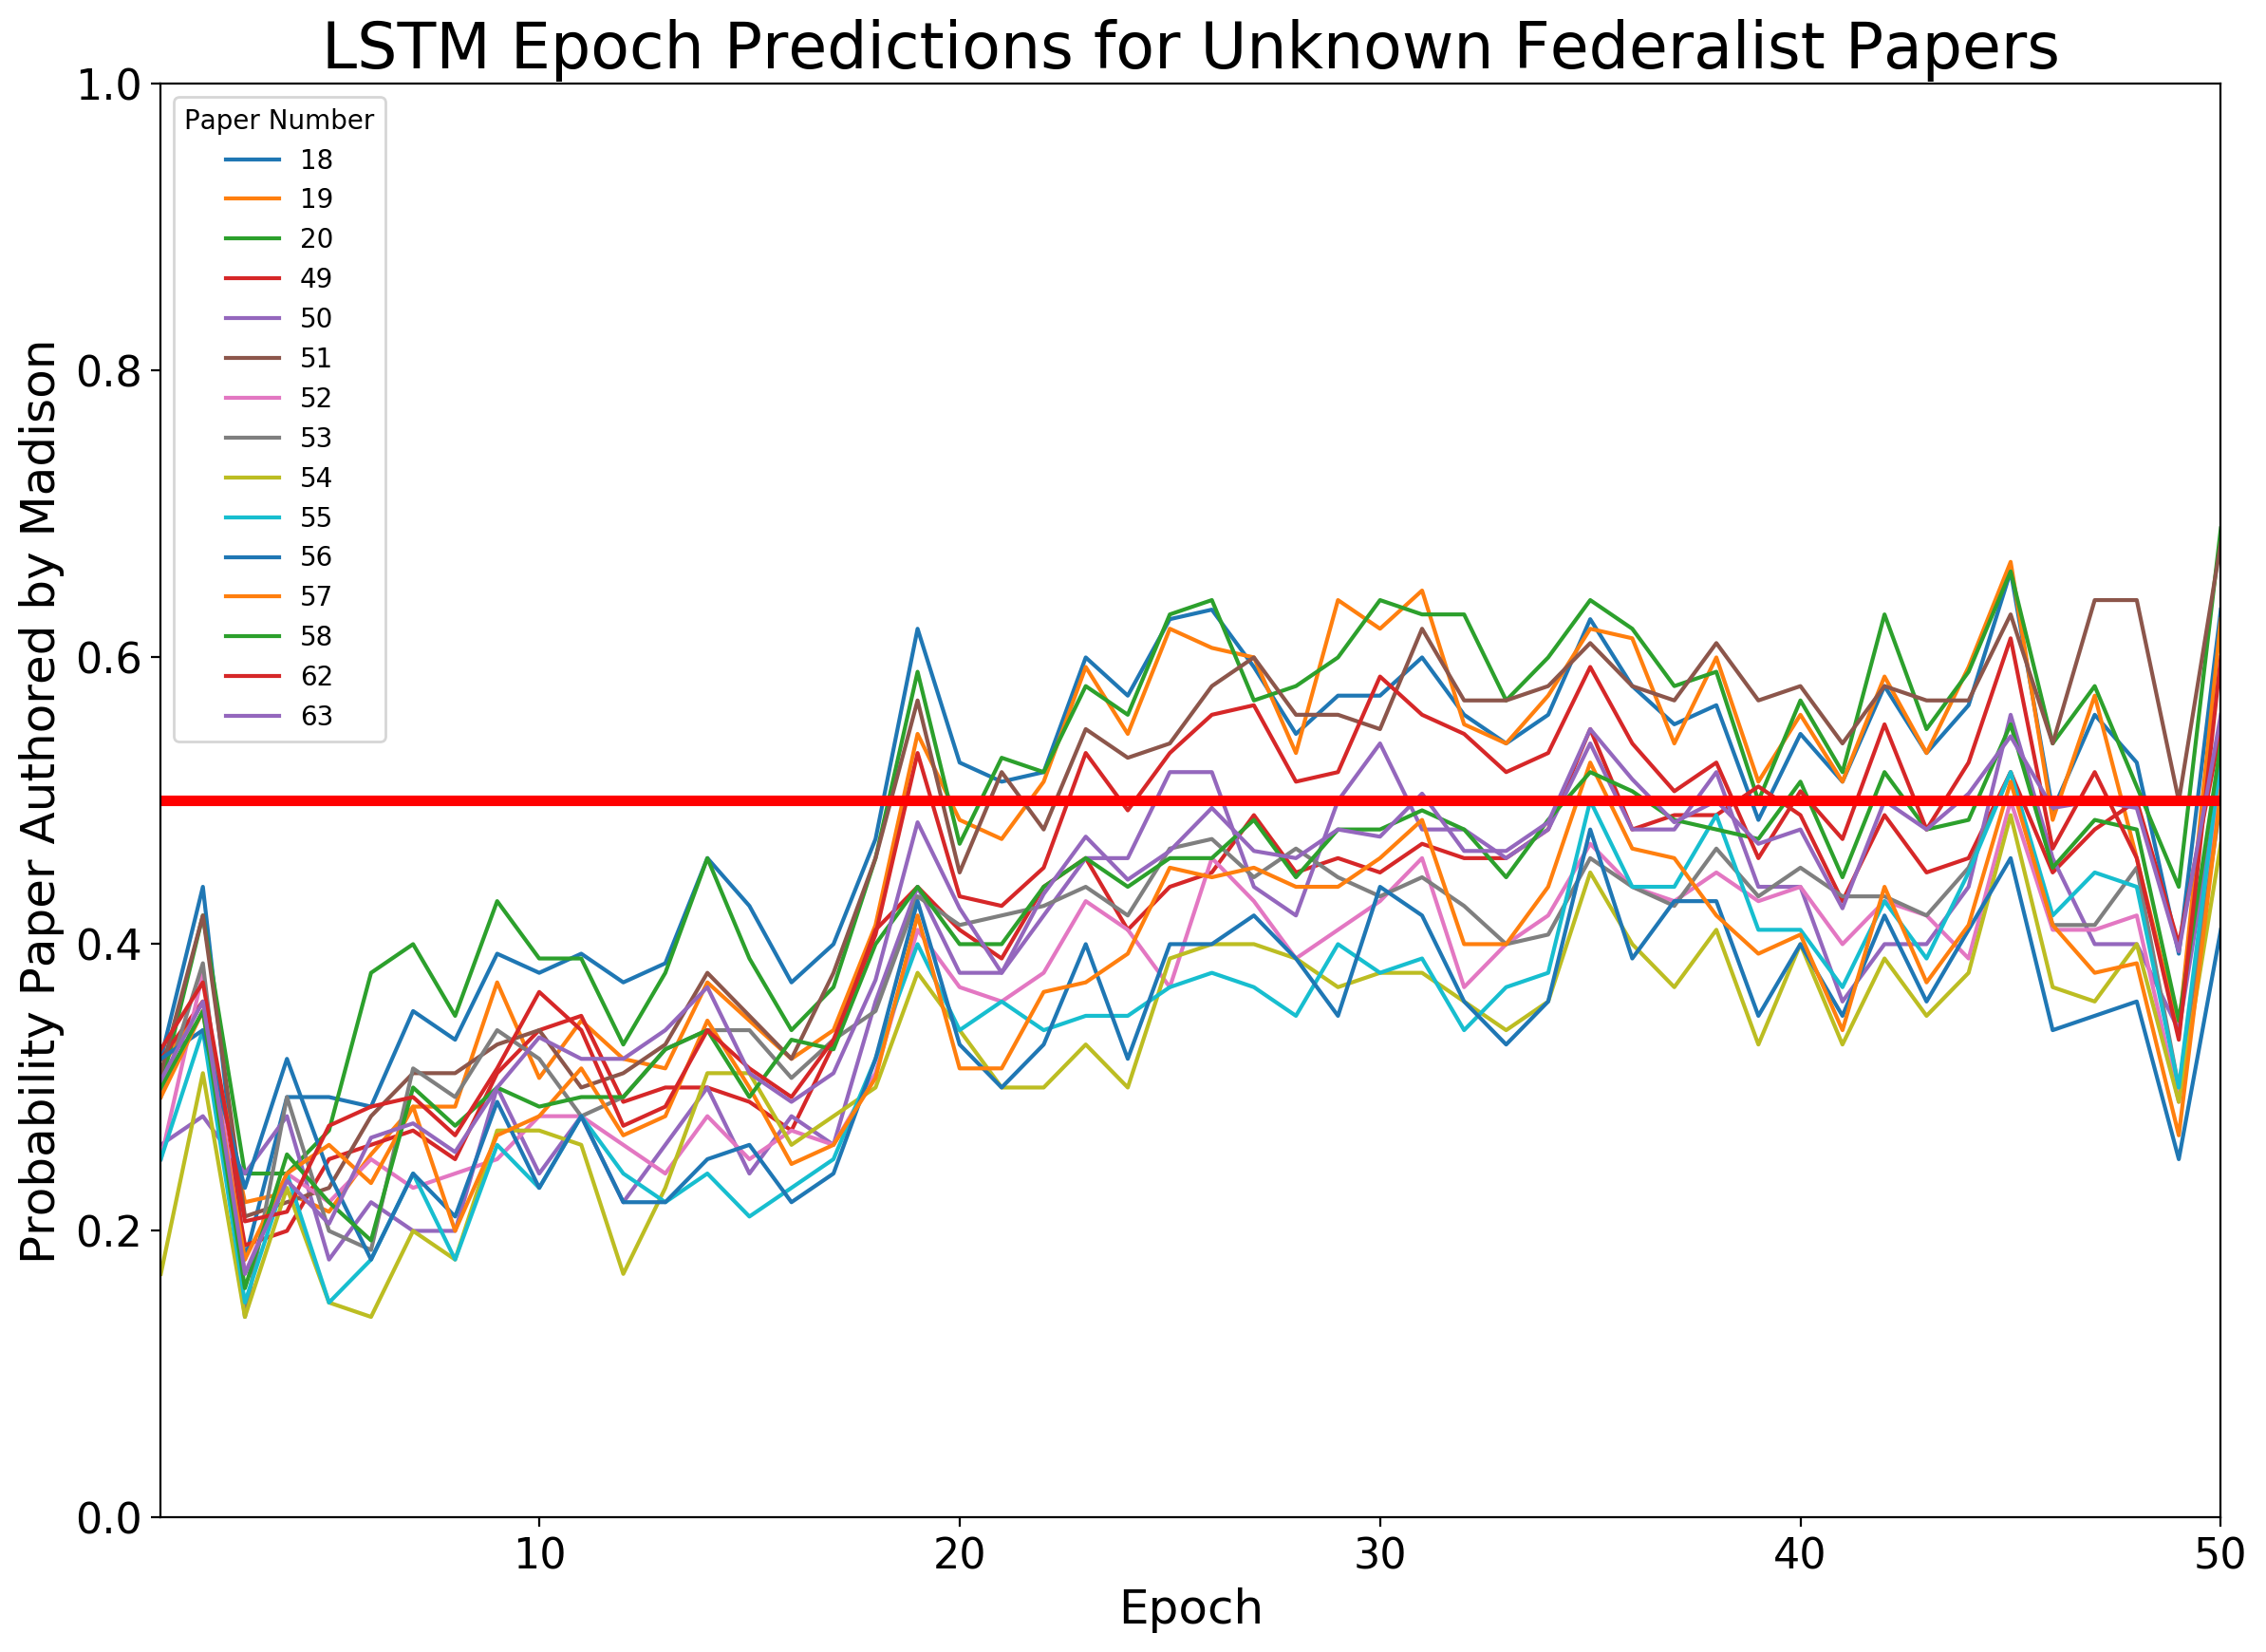
\includegraphics[width=16cm]{epoch}
	\caption{\label{epoch pred} Probability of predicting Madison as the author of each disputed paper in each epoch. Note that these predictions did not affect the training of the model. The model accuracy was based on the test set of known papers. At the same time, we saved predictions on the unknown papers for insight on the model’s behavior over the training epochs. Accuracy on the test set was used as the stopping condition for training, not results from the unknown paper predictions.}
\end{figure*}
\section{Results and Discussion}
The consensus among scholars appears to be that Madison wrote all of the disputed federalist papers (Note: many authorities believe papers 18-20 were co-written. However, even among these, the consensus appears to be that Madison wrote the majority). For this reason, we expected the results to mostly point toward Madison - and that is what we found.\\
Our initial BOW classifier, trained on the entire set of known papers, resulted in predictions where all or most of the unknown papers were predicted for Hamilton. This is also consistent with our early attempts at training an RNNLM model on the full set of known papers and with early epochs of our final RNNLM model (which was trained on the training subset of known papers). In the case of training done on the full set, we believe that the Hamilton bias in both models resulted at least in part from a class imbalance in the data - Hamilton wrote 51 of the 75 known papers. When we split out a training set from known papers, we intentionally balanced it with papers from Madison and Hamilton as best we could. This appeared to help, as our best BOW classifier (include stopwords, no tf-idf weighting) trained on the training set achieved 84.4\% accuracy on our test set of known papers. This model predicted 10 of the 15 unknown papers were authored by Madison.\\
When we trained our RNNLM model on the training set, we saw similar improvements. The model achieved greater than 95\% accuracy on the test set by epoch 50, at which point we stopped training and the model predicted that 13 of the 15 unknown papers were authored by Madison. Interestingly, the two papers predicted for Hamilton were also predicted for Hamilton under our best BOW. It could be that these papers were written by Hamilton, or that he influenced them to some degree, but that is not consistent with the historical consensus. It is more likely that there is something about these particular papers that makes them difficult to classify or similar in some way to other Hamilton papers.\\
Given the small size of our corpus, it is possible that idiosyncratic aspects of Hamilton's works had outsized effects that prevented the classifier from training properly. For example, it is possible they are getting attributed to him because they cover a similar topic only he wrote about in another paper. In such an instance, words unique to his known papers and a disputed paper might have more weight than any author writing style the BOW or RNNLM trained for.\\
Ultimately, we are pleased with the RNNLM model we trained. While it does not offer great certainty on who the authors are, it does generally agree with the baseline knowledge about who wrote the papers. We have shown that for a very specific classification task, a small corpus and an RNNLM can be enough to model authorship, but we caution against using such a model to attribute authorship to a broader set of documents.

\begin{table}[t]
	\centering
	\begin{tabular}{lr}
		\toprule
		\bf Federalist Paper &   \bf Madison \% \\
		\midrule
		No. 18 & 63 \\
		No. 19 & 63 \\
		No. 20 & 69 \\
		No. 49 & 55 \\
		No. 50 & 52 \\
		No. 51 & 68 \\
		No. 52 & 52 \\
		No. 53 & 50 \\
		No. 54 & 47 \\
		No. 55 & 53 \\
		No. 56 & 41 \\
		No. 57 & 51 \\
		No. 58 & 54 \\
		No. 62 & 60 \\
		No. 63 & 56 \\
		\bottomrule
	\end{tabular}
	\caption{\label{final results}  Predictions of RNNLM at final training epoch}
\end{table}


\section{Conclusion and Outlook}
In this paper, we showed that authorship attribution can be accomplished using a Long Short Term Model + an embedding layer and a fairly small corpus. As next steps, we would like to explore how well the CNN model~\cite{Ruder:16}~\cite{Shrestha:17} would perform on the data, as well further investigate the RNNLM with predefined features, such as those used in Jockers paper (specific word counts, punctuation counts, etc.). We still also wonder if a corpus was large enough and balanced enough, it could produce reasonable results. We used fixed length sequences of words in our model; it would also be interesting to see if variable length sequence (sentences) would yield comparable results.

\begin{thebibliography}{}
	
	\bibitem[\protect\citename{Adair}1944]{Adair:44}
	Douglass Adair.
	\newblock 1944.
	\newblock The Authorship of the Disputed Federalist Papers.
	\newblock {\em The William and Mary Quarterly}, 1(2): 97-122.

	\bibitem[\protect\citename{Ge \bgroup et al.\egroup}2016]{GeAll:16}
	 Zhenhao Ge, Yufang Sun, and Mark~J. T. Smith.
	\newblock 2016.
	\newblock Authorship Attribution Using a Neural Network  Language  Model.
	\newblock {\em Association  for  the  Advancement  of  Artificial  Intelligence}.
	
	\bibitem[\protect\citename{Ge and Sun}2016]{Ge:16}
	Zhenhao Ge and Yufang Sun.
	\newblock 2016.
	\newblock Domain Specific Author Attribution Based on Feedforward Neural Network Language Models.
	\newblock {\em International Conference on Pattern Recognition Applications and Methods}.
	
	\bibitem[\protect\citename{Hamilton \bgroup et al.\egroup}1787-1788]{Haminlton:87}
	Alexander Hamilton, John Jay, and James Madison.
	\newblock 1787-1788.
	\newblock {\em The Federalist Papers}.
	
	\bibitem[\protect\citename{Jockers and Witten}2010]{Jockers:10}
	Matthew~L. Jockers, and Daniela~M. Witten.
	\newblock 2010.
	\newblock A comparative study of machine learning methods for authorship attribution.
	\newblock {\em Literary and Linguistic Computing}, 215--223.
	
	\bibitem[\protect\citename{Mosteller and Wallace}2016]{Mosteller:63}
	Frederick Mosteller and David~L. Wallace.
	\newblock 1963.
	\newblock Inference in an Authorship Problem.
	\newblock {\em Journal of the American Statistical Association}, 58(302):275--309.
	
	\bibitem[\protect\citename{Ruder \bgroup et al.\egroup}2016]{Ruder:16}
	Sebastian Ruder, Parsa Ghaffari, and John~G. Breslin.
	\newblock 2016.
	\newblock Character-level and Multi-channel Convolutional Neural Networks for Large-scale Authorship Attribution.
	\newblock {\em CoRR}, 1609(06686).
	
	\bibitem[\protect\citename{Shrestha \bgroup et al.\egroup}2017]{Shrestha:17}
	Prasha Shrestha, Sebasti{\'a}n Sierra, Fabio A. Gonz{\'a}lez Paolo Rosso Manuel Montes-y-
	G{\'o}mez, and Thamar Solorio.
	\newblock 2017.
	\newblock Convolutional Neural Networks for Authorship Attribution of Short Texts.
	\newblock {\em Association for Computational Linguistics}, 669--674.
	
	\bibitem[\protect\citename{Stamatatos}2008]{Stamatatos:08}
	Efstathios Stamatatos.
	\newblock 2008.
	\newblock A Survey of Modern Authorship Attribution Methods.
	\newblock {\em Journal of the American Society for Information Science and Technology}, 30(3):538--556.

\end{thebibliography}

\end{document}